\documentclass[12pt,a4paper]{article}

% ─── Page Layout ───────────────────────────────────────────────────────────────
\usepackage[a4paper, margin=0.8in, headheight=14pt]{geometry}

% ─── Fonts (XeLaTeX) ───────────────────────────────────────────────────────────
\usepackage{fontspec}
\usepackage{unicode-math}
\setmainfont{TeX Gyre Pagella}
\setmonofont[Scale=0.88]{TeX Gyre Cursor}
\setmathfont{Latin Modern Math}

% ─── Packages ──────────────────────────────────────────────────────────────────
\usepackage{xcolor}
\usepackage{colortbl}
\usepackage{titlesec}
\usepackage{enumitem}
\usepackage{tabularx}
\usepackage{booktabs}
\usepackage{array}
\usepackage{amsmath}
\usepackage{tikz}
\usetikzlibrary{shapes.geometric, arrows.meta, positioning, calc, fit, decorations.pathreplacing, patterns}
\usepackage{tcolorbox}
\tcbuselibrary{skins, breakable}
\usepackage{hyperref}
\usepackage{fancyhdr}
\usepackage{graphicx}
\usepackage{microtype}
\hyphenpenalty=10000
\exhyphenpenalty=10000
\sloppy
\usepackage{caption}
\usepackage{setspace}
\usepackage{multirow}
\usepackage{tocloft}

% ─── Q&A helper ────────────────────────────────────────────────────────────────
\newcommand{\Q}[1]{\textbf{#1}\par\noindent\ignorespaces}

% ─── Colour Palette ────────────────────────────────────────────────────────────
\definecolor{myred}{RGB}{196,30,58}
\definecolor{mydark}{RGB}{30,30,50}
\definecolor{mygreen}{RGB}{14,120,80}
\definecolor{myteal}{RGB}{0,130,140}
\definecolor{myamber}{RGB}{180,100,0}
\definecolor{mypurple}{RGB}{100,30,160}
\definecolor{mygray}{RGB}{246,247,249}
\definecolor{mgframe}{RGB}{180,185,200}
\definecolor{watermark}{RGB}{145,150,170}
\definecolor{hdrred}{RGB}{250,232,235}
\definecolor{hdrgreen}{RGB}{220,244,233}
\definecolor{hdrteal}{RGB}{220,242,244}
\definecolor{hdramber}{RGB}{253,242,215}
\definecolor{hdrpurple}{RGB}{238,228,255}
\definecolor{hdrgray}{RGB}{238,240,245}
\definecolor{rowalt}{RGB}{250,251,253}

% ─── Section Formatting ────────────────────────────────────────────────────────
\titleformat{\section}
  {\large\bfseries\color{myred}}{\thesection.}{0.5em}{}
  [\vspace{1pt}{\color{myred}\rule{\linewidth}{0.8pt}}]
\titleformat{\subsection}
  {\normalsize\bfseries\color{myteal}}{\thesubsection}{0.5em}{}
\titlespacing*{\section}{0pt}{18pt}{7pt}
\titlespacing*{\subsection}{0pt}{11pt}{4pt}

% ─── Paragraph ─────────────────────────────────────────────────────────────────
\setlength{\parindent}{0pt}
\setlength{\parskip}{4pt}

% ─── TOC Styling ───────────────────────────────────────────────────────────────
\renewcommand{\cfttoctitlefont}{\large\bfseries\color{myred}}
\renewcommand{\cftaftertoctitle}{\par\noindent{\color{myred}\rule{\linewidth}{0.8pt}}}
\setlength{\cftbeforetoctitleskip}{0pt}
\setlength{\cftaftertoctitleskip}{6pt}
\renewcommand{\cftsecfont}{\normalsize\bfseries\color{mydark}}
\renewcommand{\cftsecpagefont}{\normalsize\bfseries\color{mydark}}
\renewcommand{\cftsecleader}{\cftdotfill{\cftdotsep}}
\setlength{\cftbeforesecskip}{7pt}
\renewcommand{\cftsubsecfont}{\small\color{mydark}}
\renewcommand{\cftsubsecpagefont}{\small\color{mydark}}
\setlength{\cftbeforesubsecskip}{3pt}
\setlength{\cftsubsecindent}{1.4em}

% ─── Table helpers ─────────────────────────────────────────────────────────────
\renewcommand{\arraystretch}{1.45}
\setlength{\tabcolsep}{6pt}
\arrayrulecolor{mydark}
\newcolumntype{B}[1]{>{\small\bfseries\raggedright\arraybackslash}m{#1}}
\newcolumntype{Y}{>{\small\raggedright\arraybackslash}X}
\renewcommand{\tabularxcolumn}[1]{m{#1}}

% ─── Header / Footer ───────────────────────────────────────────────────────────
\pagestyle{fancy}
\fancyhf{}
\fancyhead[L]{\small\color{myred}\textbf{EC402}\;\color{mydark}--- Analog Circuits}
\fancyhead[R]{\small\color{myteal}\textbf{Module 1 Notes}}
\fancyfoot[C]{\small\color{mydark}\thepage}
\fancyfoot[R]{\small\color{watermark}\textit{\copyright\ Biraj}}
\renewcommand{\headrulewidth}{0.5pt}
\renewcommand{\footrulewidth}{0.3pt}

% ─── Hyperref ──────────────────────────────────────────────────────────────────
\hypersetup{
  colorlinks=true, linkcolor=myteal, urlcolor=myteal,
  pdfauthor={Biraj Sarkar (CGEC)},
  pdftitle={EC402 --- Module 1 Notes: Diode Circuits, Amplifier Models and Transistor Biasing}
}

% ─── tcolorbox styles ──────────────────────────────────────────────────────────
\tcbset{
  tikzbox/.style={
    colback=mygray, colframe=mgframe, boxrule=0.6pt, arc=4pt,
    left=8pt, right=8pt, top=6pt, bottom=6pt,
    colbacktitle=mgframe, coltitle=mydark, fonttitle=\small\bfseries
  },
  defbox/.style={
    colback=hdrgreen, colframe=mygreen, boxrule=0.8pt, arc=4pt,
    left=9pt, right=9pt, top=6pt, bottom=6pt,
    colbacktitle=mygreen, coltitle=white, fonttitle=\small\bfseries
  },
  formulabox/.style={
    colback=hdrteal, colframe=myteal, boxrule=0.8pt, arc=4pt,
    left=9pt, right=9pt, top=7pt, bottom=7pt,
    colbacktitle=myteal, coltitle=white, fonttitle=\small\bfseries
  },
  examplebox/.style={
    colback=hdramber, colframe=myamber, boxrule=0.8pt, arc=4pt,
    left=9pt, right=9pt, top=6pt, bottom=6pt,
    colbacktitle=myamber, coltitle=white, fonttitle=\small\bfseries
  },
  masonbox/.style={
    colback=hdrpurple, colframe=mypurple, boxrule=0.8pt, arc=4pt,
    left=9pt, right=9pt, top=6pt, bottom=6pt,
    colbacktitle=mypurple, coltitle=white, fonttitle=\small\bfseries
  },
  exambox/.style={
    colback=hdrpurple, colframe=mypurple, boxrule=1pt, arc=5pt,
    left=10pt, right=10pt, top=8pt, bottom=8pt,
    colbacktitle=mypurple, coltitle=white, fonttitle=\bfseries,
    breakable, title after break={\textbf{Frequently Asked / Viva Questions (contd.)}}
  }
}
\tcbset{breakable}
\tcbset{after={\color{black}}}

% ─── TikZ styles ───────────────────────────────────────────────────────────────
\tikzset{
  block/.style={rectangle, draw=myteal, fill=hdrteal,
    text width=2.4cm, align=center, minimum height=0.95cm,
    font=\small, rounded corners=3pt, line width=0.7pt},
  redblock/.style={rectangle, draw=myred, fill=hdrred,
    text width=2.4cm, align=center, minimum height=0.95cm,
    font=\small, rounded corners=3pt, line width=0.7pt},
  sumjunc/.style={circle, draw=myamber, fill=hdramber,
    minimum size=0.62cm, font=\small, line width=0.8pt},
  arrow/.style={-Stealth, thick, color=mydark},
  redarrow/.style={-Stealth, thick, color=myred},
  line/.style={thick, color=mydark}
}

\begin{document}

% ─── Title Page ───────────────────────────────────────────────────────────────
\begin{center}
  {\LARGE\bfseries\color{myred} EC402 --- Analog Circuits}\\[5pt]
  {\normalsize\color{mydark} Semester IV \quad$\bullet$\quad 3L:0T:0P \quad$\bullet$\quad 3 Credits}\\[3pt]
  {\normalsize\color{myteal}\textbf{Module 1 Exam Notes: Diode Circuits, Amplifier Models and Transistor Biasing}}\\[3pt]
  {\small\color{mydark} CGEC \;$|$\; B.Tech ECE (2023--27) \;$|$\; \textit{Biraj Sarkar}}
\end{center}
\vspace{2pt}
\noindent{\color{myred}\rule{\linewidth}{1.5pt}}
\vspace{2pt}

\hypersetup{linkcolor=mydark}
\tableofcontents
\hypersetup{linkcolor=myteal}
\newpage

\section{Diode Circuits: Rectifiers, Filters, Clippers and Clampers}

\begin{tcolorbox}[defbox, title={Rectifier Fundamentals}]
A \textbf{rectifier} is a non-linear circuit converting alternating voltage ($ac$) to unidirectional pulsating direct voltage ($dc$) utilizing the unilateral conduction of $p$-$n$ junction diodes. The performance of rectifiers is governed by rectification efficiency $\eta$, ripple factor $\gamma$, Transformer Utilization Factor ($\mathrm{TUF}$), and Peak Inverse Voltage ($\mathrm{PIV}$).
\end{tcolorbox}

\subsection{Half-Wave and Full-Wave Rectifiers}
Consider an input $v_i(t) = V_m\sin(\omega t)$ applied across a load resistance $R_L$ with diode forward resistance $r_f$.

\begin{enumerate}[leftmargin=1.5em, itemsep=3pt]
  \item \textbf{Half-Wave Rectifier (HWR)}: Conducts only during positive half cycles ($0 \le \omega t \le \pi$):
  \[
  \begin{aligned}
  I_{dc} &= \frac{1}{2\pi}\int_0^\pi I_m\sin\theta\,d\theta = \frac{I_m}{\pi},\qquad V_{dc} = I_{dc}R_L = \frac{V_m}{\pi},\\
  I_{rms} &= \sqrt{\frac{1}{2\pi}\int_0^\pi I_m^2\sin^2\theta\,d\theta} = \frac{I_m}{2},\qquad V_{rms} = \frac{V_m}{2}.
  \end{aligned}
  \]
  \item \textbf{Full-Wave Rectifier (Center-Tapped and Bridge)}: Conducts during both half cycles:
  \[
  \begin{aligned}
  I_{dc} &= \frac{1}{\pi}\int_0^\pi I_m\sin\theta\,d\theta = \frac{2I_m}{\pi},\qquad V_{dc} = \frac{2V_m}{\pi},\\
  I_{rms} &= \sqrt{\frac{1}{\pi}\int_0^\pi I_m^2\sin^2\theta\,d\theta} = \frac{I_m}{\sqrt{2}},\qquad V_{rms} = \frac{V_m}{\sqrt{2}}.
  \end{aligned}
  \]
\end{enumerate}

\begin{tcolorbox}[formulabox, title={Performance Metrics of Rectifiers}]
\begin{enumerate}[leftmargin=1.5em, itemsep=2pt]
  \item \textbf{Ripple Factor ($\gamma$)}: Ratio of effective $ac$ component to the average $dc$ level:
  \[
  \gamma = \frac{V_{ac,rms}}{V_{dc}} = \sqrt{\left(\frac{I_{rms}}{I_{dc}}\right)^2 - 1}.
  \]
  For HWR: $\gamma = \sqrt{(\pi/2)^2 - 1} \approx 1.21$. For FWR: $\gamma = \sqrt{(\pi/(2\sqrt{2}))^2 - 1} \approx 0.482$.
  \item \textbf{Rectification Efficiency ($\eta$)}: Ratio of $dc$ output power to total $ac$ input power:
  \[
  \eta = \frac{P_{dc}}{P_{ac}} = \frac{I_{dc}^2 R_L}{I_{rms}^2 (R_L + r_f)}.
  \]
  For HWR: $\eta_{\max} = \frac{4}{\pi^2} \approx 40.6\%$. For FWR: $\eta_{\max} = \frac{8}{\pi^2} \approx 81.2\%$.
  \item \textbf{Transformer Utilization Factor ($\mathrm{TUF}$)}: $\mathrm{TUF} = P_{dc} / V_{\text{rated}}I_{\text{rated}}$.
  $\mathrm{TUF}_{\mathrm{HWR}} = 0.287$, $\mathrm{TUF}_{\mathrm{FWR,Center}} = 0.693$, $\mathrm{TUF}_{\mathrm{Bridge}} = 0.812$.
  \item \textbf{Peak Inverse Voltage ($\mathrm{PIV}$)}: Maximum reverse bias voltage appearing across a non-conducting diode:
  $\mathrm{PIV}_{\mathrm{HWR}} = V_m$, $\mathrm{PIV}_{\mathrm{Center-Tapped}} = 2V_m$, $\mathrm{PIV}_{\mathrm{Bridge}} = V_m$.
\end{enumerate}
\end{tcolorbox}

\par\vspace{6pt}\noindent
\begin{tabularx}{\linewidth}{|B{3.4cm}|Y|Y|Y|}
\hline
\textbf{Parameter} & \textbf{Half-Wave Rectifier} & \textbf{Center-Tapped FWR} & \textbf{Bridge Rectifier} \\
\hline
\textbf{Number of Diodes} & 1 & 2 & 4 \\
\hline
\textbf{$dc$ Voltage ($V_{dc}$)} & $V_m/\pi \approx 0.318 V_m$ & $2V_m/\pi \approx 0.636 V_m$ & $2V_m/\pi \approx 0.636 V_m$ \\
\hline
\textbf{Ripple Factor ($\gamma$)} & $1.21$ ($121\%$ ripple) & $0.482$ ($48.2\%$ ripple) & $0.482$ ($48.2\%$ ripple) \\
\hline
\textbf{Efficiency ($\eta_{\max}$)}& $40.6\%$ & $81.2\%$ & $81.2\%$ \\
\hline
\textbf{Ripple Frequency} & $f_{in}$ ($50\,\mathrm{Hz}$) & $2f_{in}$ ($100\,\mathrm{Hz}$) & $2f_{in}$ ($100\,\mathrm{Hz}$) \\
\hline
\textbf{Peak Inverse Voltage} & $V_m$ & $2V_m$ & $V_m$ \\
\hline
\textbf{Center-Tap Required}& No & Yes (bulky transformer) & No \\
\hline
\end{tabularx}
\par\vspace{12pt}

\subsection{Power Supply Smoothing Filters}
Smoothing filters suppress $ac$ ripple harmonics leaving pure $dc$:
\begin{enumerate}[leftmargin=1.5em, itemsep=2pt]
  \item \textbf{Shunt Capacitor Filter ($C$-Filter)}: Capacitor charges to $V_m$ on peaks and discharges slowly into $R_L$ with time constant $R_L C \gg T/2$. Ripple factor for FWR: $\gamma \approx \frac{1}{4\sqrt{3} f R_L C}$.
  \item \textbf{Series Inductor Filter ($L$-Filter)}: Opposes sudden current changes: $\gamma \approx \frac{R_L}{3\sqrt{2}\omega L}$. Suitable for heavy loads (small $R_L$).
  \item \textbf{Choke-Input ($LC$) Filter}: Combines series $L$ and shunt $C$: $\gamma \approx \frac{\sqrt{2}}{3}\frac{X_C}{X_L} = \frac{1}{6\sqrt{2}\omega^2 L C}$, independent of load resistance $R_L$. Critical inductance: $L_c \ge R_L / (3\omega)$.
  \item \textbf{$\pi$-Filter ($CLC$-Filter)}: Yields lowest ripple: $\gamma \approx \frac{\sqrt{2}}{8\omega^3 C_1 C_2 L R_L}$, but high diode surge current.
\end{enumerate}

\subsection{Clippers (Limiters) and Clampers (DC Restorers)}
\begin{itemize}[leftmargin=1.5em, itemsep=3pt]
  \item \textbf{Clippers}: Waveform-shaping circuits that remove portions of an applied signal above or below preset reference levels without distorting the remaining part. Implemented as series clippers (diode in series with signal path) or shunt clippers (diode in parallel across load).
  \item \textbf{Two-Level (Slicer) Clipper}: Two diodes biased with opposite reference voltages ($V_{R1}, V_{R2}$) clip both positive and negative peaks, generating trapezoidal or square waves from a sine wave.
  \item \textbf{Clampers}: Circuits that shift the entire waveform up or down to a different $dc$ level without altering the peak-to-peak amplitude. Requires a diode, capacitor, and resistor satisfying $R_L C \ge 10T$.
  \item \textbf{Clamping Theorem}: At steady state, ratio of area under positive curve ($A_+$) to negative curve ($A_-$) equals ratio of forward resistance to load resistance: $A_+ / A_- = r_f / R_L$.
\end{itemize}

\begin{tcolorbox}[tikzbox, unbreakable, title={Diode Clipper and Clamper Topologies}]
\centering
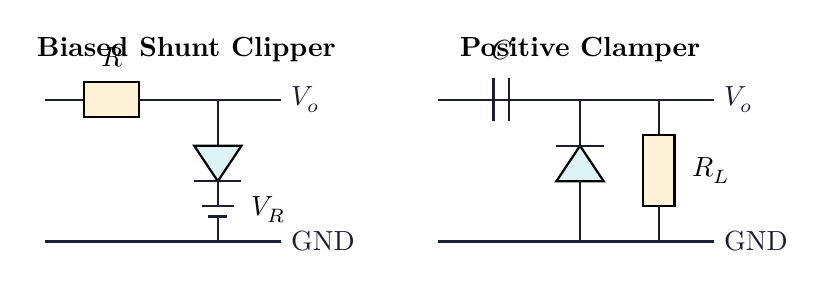
\begin{tikzpicture}[x=1cm,y=0.9cm]
  % Shunt Clipper
  \node[above] at (1.8,2.4) {\bfseries Biased Shunt Clipper};
  \draw[line] (0,2)--(1.5,2);
  \draw[thick,fill=hdramber] (0.5,1.75) rectangle (1.2,2.25);
  \node[above=2pt] at (0.85,2.25) {$R$};
  \draw[line] (1.2,2)--(3,2) node[right] {$V_o$};
  \draw[line] (0,0)--(3,0) node[right] {GND};
  \draw[line] (2.2,2)--(2.2,1.35);
  \draw[thick,fill=hdrteal] (1.9,1.35)--(2.5,1.35)--(2.2,0.85)--cycle;
  \draw[line] (1.9,0.85)--(2.5,0.85);
  \draw[line] (2.2,0.85)--(2.2,0.5);
  \draw[line] (2.0,0.5)--(2.4,0.5);
  \draw[line] (2.08,0.35)--(2.32,0.35);
  \draw[line] (2.2,0.35)--(2.2,0);
  \node[right=3pt] at (2.4,0.45) {$V_R$};

  % Positive Clamper
  \node[above] at (6.8,2.4) {\bfseries Positive Clamper};
  \draw[line] (5,2)--(6,2);
  \draw[line] (5.7,2.3)--(5.7,1.7);
  \draw[line] (5.9,2.3)--(5.9,1.7);
  \node[above=3pt] at (5.8,2.3) {$C$};
  \draw[line] (5.9,2)--(8.5,2) node[right] {$V_o$};
  \draw[line] (5,0)--(8.5,0) node[right] {GND};
  \draw[line] (6.8,2)--(6.8,1.35);
  \draw[thick,fill=hdrteal] (6.5,0.85)--(7.1,0.85)--(6.8,1.35)--cycle;
  \draw[line] (6.5,1.35)--(7.1,1.35);
  \draw[line] (6.8,0.85)--(6.8,0);
  \draw[line] (7.8,2)--(7.8,1.5);
  \draw[thick,fill=hdramber] (7.6,0.5) rectangle (8.0,1.5);
  \node[right=3pt] at (8.0,1.0) {$R_L$};
  \draw[line] (7.8,0.5)--(7.8,0);
\end{tikzpicture}\par
\small Shunt clipper limits peaks above $V_R + V_D$. The positive clamper shifts the signal upwards so that its negative peaks rest at $0\,\mathrm{V}$.
\end{tcolorbox}

\section{Two-Port Amplifier Models and Loading Effects}

\begin{tcolorbox}[defbox, title={The Four Fundamental Amplifier Models}]
Amplifiers are linear two-port networks characterized by input resistance $R_i$, open-circuit or short-circuit gain parameter, and output resistance $R_o$:
\begin{enumerate}[leftmargin=1.5em, itemsep=2pt]
  \item \textbf{Voltage Amplifier}: $V_o = A_{vo} V_i$. Ideal: $R_i \to \infty$, $R_o = 0$.
  \item \textbf{Current Amplifier}: $I_o = A_{is} I_i$. Ideal: $R_i = 0$, $R_o \to \infty$.
  \item \textbf{Transconductance Amplifier}: $I_o = G_m V_i$. Ideal: $R_i \to \infty$, $R_o \to \infty$.
  \item \textbf{Transresistance Amplifier}: $V_o = R_m I_i$. Ideal: $R_i = 0$, $R_o = 0$.
\end{enumerate}
\end{tcolorbox}

\subsection{Source and Load Resistance Loading Effects}
When connected between an actual source ($V_s, R_s$) and a real load $R_L$:
\[
V_i = V_s \left(\frac{R_i}{R_s + R_i}\right),\qquad
V_o = A_{vo} V_i \left(\frac{R_L}{R_o + R_L}\right) = A_{vo} V_s \left(\frac{R_i}{R_s + R_i}\right)\left(\frac{R_L}{R_o + R_L}\right).
\]
Effective voltage gain $A_v = V_o/V_s$ drops below intrinsic gain $A_{vo}$ due to input voltage division (when $R_s \not\ll R_i$) and output loading (when $R_L \not\gg R_o$).

\begin{tcolorbox}[examplebox, title={Amplifier Loading Effect Calculation}]
A voltage amplifier has $R_i = 100\,\mathrm{k}\Omega$, $R_o = 50\,\Omega$, and $A_{vo} = 200$. It is driven by a source with $R_s = 25\,\mathrm{k}\Omega$ and drives a load $R_L = 100\,\Omega$.
\[
\begin{aligned}
\text{Input attenuation factor:}\quad \alpha_i &= \frac{R_i}{R_s + R_i} = \frac{100}{25 + 100} = 0.8,\\
\text{Output loading factor:}\quad \alpha_o &= \frac{R_L}{R_o + R_L} = \frac{100}{50 + 100} = 0.667,\\
\text{Overall voltage gain:}\quad A_v &= \frac{V_o}{V_s} = A_{vo}\cdot\alpha_i\cdot\alpha_o = 200(0.8)(0.667) \approx 106.7.
\end{aligned}
\]
Loading degrades the effective amplification from $200$ to $106.7$ ($46.6\%$ loss).
\end{tcolorbox}

\section{Biasing Schemes and Stability Analysis for BJT and FET}

\begin{tcolorbox}[defbox, title={Operating Point ($Q$-Point) and Stability}]
To amplify linear $ac$ signals without clipping, transistors must be biased in the \textbf{Active Region} (BJT: forward-biased emitter junction, reverse-biased collector junction; FET: pinched-off saturation region). The operating point $Q(V_{CEQ}, I_{CQ})$ represents the steady-state $dc$ voltages and currents.
\end{tcolorbox}

\subsection{BJT Biasing Configurations and Stability Factors}
Variations in temperature $T$ cause drift in reverse saturation current $I_{CO}$ (doubles every $10^\circ\mathrm{C}$ rise), base-emitter voltage $V_{BE}$ (decreases by $2.5\,\mathrm{mV/^\circ C}$), and current gain $\beta$. Stability factors define the sensitivity:
\[
S = \frac{\partial I_C}{\partial I_{CO}},\qquad
S' = \frac{\partial I_C}{\partial V_{BE}},\qquad
S'' = \frac{\partial I_C}{\partial \beta}.
\]
General relation: $I_C = \beta I_B + (1+\beta)I_{CO}$. Differentiating with respect to $I_C$:
\[
S = \frac{1 + \beta}{1 - \beta \left(\dfrac{\partial I_B}{\partial I_C}\right)}.
\]

\begin{enumerate}[leftmargin=1.5em, itemsep=3pt]
  \item \textbf{Fixed Bias}: $I_B = (V_{CC} - V_{BE})/R_B$. Since $\partial I_B/\partial I_C = 0$, $S = 1+\beta$. Highly unstable ($S \approx 100$--$300$); thermal runaway occurs readily.
  \item \textbf{Collector-to-Base Feedback Bias}: $I_B = (V_{CC} - V_{BE} - I_C R_C)/(R_B + R_C)$. Provides negative feedback: $\partial I_B/\partial I_C = -R_C/(R_B+R_C) < 0$, giving $S = \frac{1+\beta}{1 + \beta R_C/(R_B+R_C)} < 1+\beta$.
  \item \textbf{Voltage Divider Bias (Self-Bias / Emitter Bias)}: Most robust topology. Applying Thevenin's theorem at the base:
  \[
  V_{th} = V_{CC}\left(\frac{R_2}{R_1+R_2}\right),\qquad R_{th} = R_1 \parallel R_2.
  \]
  Loop equation: $V_{th} = I_B R_{th} + V_{BE} + I_E R_E \approx I_B R_{th} + V_{BE} + (I_B + I_C)R_E$.
  \[
  I_B = \frac{V_{th} - V_{BE} - I_C R_E}{R_{th} + R_E} \implies \frac{\partial I_B}{\partial I_C} = -\frac{R_E}{R_{th} + R_E}.
  \]
  Substituting into the stability factor formula:
  \[
  S = (1+\beta)\frac{1 + R_{th}/R_E}{1+\beta + R_{th}/R_E}.
  \]
  \textit{Condition for Excellent Stability}: If $R_{th}/R_E \ll 1$, then $S \to 1$ (perfect stability independent of $\beta$). Practical rule: $R_{th} \le 0.1(1+\beta)R_E$ and $I_{\mathrm{divider}} \ge 10 I_B$.
\end{enumerate}

\subsection{Thermal Runaway Avoidance}
Collector power dissipation is $P_C \approx V_{CE} I_C$. Temperature rise $\Delta T = \theta P_C$ (where $\theta$ is thermal resistance in $^\circ\mathrm{C/W}$). A cumulative cycle occurs: $T \uparrow \implies I_{CO} \uparrow \implies I_C \uparrow \implies P_C \uparrow \implies T \uparrow$ until destructive breakdown occurs.
\begin{tcolorbox}[formulabox, title={Condition to Prevent Thermal Runaway}]
Thermal runaway is completely prevented if the rate of heat dissipation exceeds the rate of heat generation:
\[
\frac{\partial P_C}{\partial T_j} < \frac{1}{\theta} \iff V_{CE} < \frac{V_{CC}}{2}.
\]
In practice, designing $V_{CEQ} \le V_{CC}/2$ ensures inherent unconditional thermal stability.
\end{tcolorbox}

\subsection{FET Biasing Schemes (JFET and MOSFET)}
For JFETs and depletion MOSFETs, drain current follows Shockley's equation: $I_D = I_{DSS}(1 - V_{GS}/V_P)^2$.
\begin{itemize}[leftmargin=1.5em, itemsep=2pt]
  \item \textbf{Self-Bias}: Gate grounded ($V_G = 0$) via high resistor $R_G$ ($1\,\mathrm{M}\Omega$). Source resistor $R_S$ develops $V_S = I_D R_S$, producing $V_{GS} = -I_D R_S$. The operating point is the intersection of the transfer curve with the $dc$ bias line $I_D = -V_{GS}/R_S$.
  \item \textbf{Voltage Divider Bias}: $V_G = V_{DD}[R_2/(R_1+R_2)]$. Then $V_{GS} = V_G - I_D R_S$, stabilizing $I_{DQ}$ against device parameter variations ($I_{DSS}$ and $V_P$ spreads).
\end{itemize}

\section{Small-Signal Analysis and Low-Frequency Transistor Models}

\subsection{Low-Frequency BJT Models \texorpdfstring{($h$-Parameter and Hybrid-$\pi$)}{(h-Parameter and Hybrid-pi)}}
For small $ac$ excursions around the $Q$-point:
\begin{itemize}[leftmargin=1.5em, itemsep=2pt]
  \item \textbf{$h$-Parameter Model}: $v_1 = h_i i_1 + h_r v_2$, $i_2 = h_f i_1 + h_o v_2$. For CE: $h_{ie}$ (input resistance), $h_{re}$ (reverse voltage feedback), $h_{fe} = \beta$ (forward current gain), $h_{oe}$ (output conductance).
  \item \textbf{Hybrid-$\pi$ Model}: Transconductance $g_m = I_C/V_T$ (where $V_T = k T/q \approx 26\,\mathrm{mV}$ at room temp), base resistance $r_\pi = \beta/g_m = \beta V_T/I_C$, output resistance $r_o = V_A/I_C$ (where $V_A$ is the Early voltage), and emitter intrinsic resistance $r_e = \alpha/g_m \approx V_T/I_E$.
\end{itemize}

\subsection{BJT Amplifier Configurations (CE, CB, CC)}
\begin{tcolorbox}[defbox, title={Common-Terminal BJT Configurations}]
An amplifier configuration is named for the transistor terminal shared by the input and output signal paths. In \textbf{common emitter (CE)}, the input is at the base and the output at the collector. In \textbf{common base (CB)}, the input is at the emitter and the output at the collector. In \textbf{common collector (CC)}, the input is at the base and the output at the emitter.
\end{tcolorbox}

\begin{tcolorbox}[formulabox, title={Analytical Small-Signal Expressions for BJT Amplifiers}, title after break={BJT Amplifier Expressions (contd.)}]
\begin{enumerate}[leftmargin=1.8em, itemsep=8pt]
  \item \textbf{Common Emitter (CE) with Bypass $C_E$}:
  \[
  \begin{aligned}
  A_v &= -g_m (R_C \parallel R_L)
       = -\frac{\beta (R_C \parallel R_L)}{r_\pi}
       \approx -\frac{R_C \parallel R_L}{r_e}, \\[3pt]
  R_i &= R_B \parallel r_\pi, \\[3pt]
  R_o &= R_C \parallel r_o.
  \end{aligned}
  \]
  Provides high inverting voltage gain ($180^\circ$ phase inversion) and high current gain.
  \item \textbf{Common Emitter with Unbypassed Emitter Resistor $R_E$}:
  \[
  \begin{aligned}
  A_v &\approx -\frac{R_C \parallel R_L}{r_e + R_E}, \\[3pt]
      &\approx -\frac{R_C \parallel R_L}{R_E}
        \quad \text{when } R_E \gg r_e, \\[3pt]
  R_i &= R_B \parallel \left[r_\pi + (1+\beta)R_E\right].
  \end{aligned}
  \]
  Degeneration stabilizes voltage gain against temperature and parameter drift at the cost of reduced gain.
  \item \textbf{Common Collector (CC / Emitter Follower)}:
  Let $R_E' = R_E \parallel R_L$ be the loaded emitter resistance and
  $R_s' = R_s \parallel R_B$ be the resistance seen from the base with
  the input source set to zero.
  \[
  \begin{aligned}
  A_v &= \frac{(1+\beta)R_E'}{r_\pi + (1+\beta)R_E'} \approx 1, \\[3pt]
  R_i &= R_B \parallel \left[r_\pi + (1+\beta)R_E'\right], \\[3pt]
  R_o &= R_E \parallel \left(\frac{r_\pi + R_s'}{1+\beta}\right).
  \end{aligned}
  \]
  The near-unity gain, high input resistance and low output resistance
  make this stage useful as a non-inverting buffer.
  \item \textbf{Common Base (CB)}:
  \[
  \begin{aligned}
  A_v &= +g_m (R_C \parallel R_L), & A_i &\approx \alpha \approx 1, \\[3pt]
  R_i &\approx r_e \parallel R_E, & R_o &\approx R_C.
  \end{aligned}
  \]
  For $R_E \gg r_e$, the input resistance is close to $r_e$.
  The stage is non-inverting and is used in high-frequency RF amplifiers.
\end{enumerate}
\end{tcolorbox}

\par\vspace{6pt}\noindent
\begin{tabularx}{\linewidth}{|B{3.2cm}|Y|Y|Y|}
\hline
\textbf{Parameter} & \textbf{Common Emitter (CE)} & \textbf{Common Collector (CC)} & \textbf{Common Base (CB)} \\
\hline
\textbf{Voltage Gain ($A_v$)} & High ($\sim -100$ to $-500$) & Low ($\approx 1$, non-inverting) & High ($\sim +100$ to $+500$) \\
\hline
\textbf{Current Gain ($A_i$)} & High ($\sim \beta \approx 100$) & Highest ($\sim 1+\beta \approx 101$)& Low ($\sim \alpha \approx 0.99$) \\
\hline
\textbf{Input Resistance ($R_i$)}& Moderate ($\sim 1\,\mathrm{k}\Omega$--$5\,\mathrm{k}\Omega$) & Very High ($\sim 100\,\mathrm{k}\Omega$--$500\,\mathrm{k}\Omega$) & Very Low ($\sim 20\,\Omega$--$50\,\Omega$) \\
\hline
\textbf{Output Resistance ($R_o$)}& Moderate ($\sim 10\,\mathrm{k}\Omega$--$50\,\mathrm{k}\Omega$)& Very Low ($\sim 10\,\Omega$--$50\,\Omega$) & High ($\sim 100\,\mathrm{k}\Omega$--$1\,\mathrm{M}\Omega$) \\
\hline
\textbf{Phase Shift} & $180^\circ$ (inverting) & $0^\circ$ (in-phase) & $0^\circ$ (in-phase) \\
\hline
\textbf{Primary Application}& Voltage \& Power Amplification & Impedance Matching / Buffer & High-Frequency RF Amplifier \\
\hline
\end{tabularx}
\par\vspace{12pt}

\subsection{Multistage Amplifiers (Low Frequency)}
When multiple amplifier stages are cascaded ($n$ stages):
\[
A_v = A_{v1} \cdot A_{v2} \cdots A_{vn},\qquad
R_{in} = R_{in1},\qquad
R_{out} = R_{out,n}.
\]
Stage 2 acts as the load resistance for Stage 1 ($R_{L1} = R_{in2}$), which significantly attenuates intermediate gains (loading effect). Three primary coupling schemes are used:
\begin{itemize}[leftmargin=1.5em, itemsep=2pt]
  \item \textbf{RC Coupling}: Blocks $dc$ bias voltages between stages; flat audio response; poor low-frequency gain due to coupling capacitor reactance.
  \item \textbf{Transformer Coupling}: Perfect impedance matching via turns ratio $(N_p/N_s)^2$; high $dc$ power efficiency; bulky, expensive, and poor high-frequency response.
  \item \textbf{Direct Coupling}: No capacitors; passes $dc$ and sub-hertz signals; mandatory in integrated circuits (ICs); susceptible to $dc$ operating point drift.
\end{itemize}

\newpage

% ─── Quick Revision Page ───────────────────────────────────────────────────────
\begin{center}
  {\large\bfseries\color{myred} Quick Revision --- Module 1}\\[3pt]
  {\small\color{mydark} Rectifiers, BJT Biasing and Small-Signal Amplifiers $|$ EC402}
\end{center}
\noindent{\color{myred}\rule{\linewidth}{1.2pt}}
\vspace{4pt}

\begin{tcolorbox}[formulabox, title={Key Formulas at a Glance}]
\small
\renewcommand{\arraystretch}{1.35}
\setlength{\tabcolsep}{5pt}
\noindent\begin{tabularx}{\linewidth}{B{4.1cm}Y}
Rectifier DC Voltages & $V_{dc,\mathrm{HWR}} = V_m/\pi$ \newline $V_{dc,\mathrm{FWR}} = 2V_m/\pi$ \\[3pt]
Ripple Factor ($\gamma$) & $\gamma = \sqrt{(I_{rms}/I_{dc})^2 - 1}$ \newline $\gamma_{\mathrm{HWR}} \approx 1.21$ \newline $\gamma_{\mathrm{FWR}} = 0.482$ \\[3pt]
Rectifier Efficiency ($\eta$) & $\eta_{\mathrm{HWR}} = 40.6\%$ \newline $\eta_{\mathrm{FWR}} = 81.2\%$ \\[3pt]
$C$-Filter Ripple Factor & $\gamma = \frac{1}{4\sqrt{3} f R_L C}$ (Full-wave) \\[3pt]
BJT Stability Factor ($S$) & $S = (1+\beta)\frac{1 + R_{th}/R_E}{1+\beta + R_{th}/R_E}$ \newline Condition: $R_{th} \ll R_E \implies S \to 1$ \\[3pt]
Thermal Runaway Condition & Stable if $V_{CE} < V_{CC}/2$ or $\frac{\partial P_C}{\partial T_j} < \frac{1}{\theta}$ \\[3pt]
Transconductance ($g_m$) & $g_m = \frac{I_C}{V_T} \approx \frac{I_C}{26\,\mathrm{mV}}$ \newline $r_\pi = \frac{\beta}{g_m}$ \newline $r_e = \frac{\alpha}{g_m} \approx \frac{26\,\mathrm{mV}}{I_E}$ \\[3pt]
CE Voltage Gain & $A_v = -g_m (R_C \parallel R_L) \approx -\frac{R_C \parallel R_L}{r_e}$ (with bypass $C_E$) \\[3pt]
CC Voltage Gain \& $R_o$ & $A_v \approx 1$ \newline $R_o = R_E \parallel \left(\frac{r_\pi + R_s'}{1+\beta}\right)$ \newline $R_s^\prime = R_s \parallel R_B$ \\[3pt]
Multistage Gain & $A_{v,\mathrm{total}} = A_{v1} \times A_{v2} \times \dots \times A_{vn}$ \newline $A_{v,\mathrm{dB}} = \sum A_{vk,\mathrm{dB}}$
\end{tabularx}\par
\end{tcolorbox}

\begin{tcolorbox}[defbox, title={One-Line Definitions}, title after break={One-Line Definitions (contd.)}]
\small
\interlinepenalty=10000
\begin{itemize}[leftmargin=1.5em, topsep=2pt, itemsep=4pt]
  \item \textbf{Ripple Factor}: The RMS value of the AC component of a rectifier output divided by the magnitude of its DC value.
  \item \textbf{Peak Inverse Voltage (PIV)}: The largest reverse voltage across a diode while it is off.
  \item \textbf{Transformer Utilization Factor (TUF)}: The ratio of $dc$ power delivered to the load to the $ac$ volt-ampere rating of the transformer secondary.
  \item \textbf{Clamping Circuit}: A circuit that shifts the DC level of a waveform while ideally keeping its peak-to-peak amplitude the same.
  \item \textbf{Operating Point ($Q$-Point)}: The steady DC collector current $I_{CQ}$ and collector--emitter voltage $V_{CEQ}$ set by the bias circuit with no input signal.
  \item \textbf{Stability Factor ($S$)}: The change in collector current per unit change in leakage current with $\beta$ and $V_{BE}$ held fixed: $S=\partial I_C/\partial I_{CO}$.
  \item \textbf{Thermal Runaway}: A cycle in which a rise in transistor temperature increases leakage current and power dissipation, causing further heating.
  \item \textbf{Transconductance ($g_m$)}: The change in BJT collector current per unit change in base--emitter voltage at the operating point. In the small-signal model, $g_m=I_C/V_T$ and its unit is the siemens.
  \item \textbf{Emitter Follower}: A common-collector BJT amplifier whose emitter output follows the base input with nearly unity voltage gain. Its high input and low output resistances make it useful as a buffer.
\end{itemize}
\end{tcolorbox}

\begin{tcolorbox}[exambox, title={Frequently Asked / Viva Questions}]
\begin{enumerate}[topsep=0pt, label=\textbf{Q\arabic*.}, itemsep=5pt]
  \item \Q{Why is the ripple factor of a full-wave rectifier less than half that of a half-wave rectifier?}
  Because the FWR conducts on both half cycles, doubling fundamental ripple frequency ($2f$) and halving the period during which the load draws from the capacitor, reducing ripple from $1.21$ to $0.482$.

  \item \Q{Why is the bridge rectifier preferred over the center-tapped full-wave rectifier?}
  The bridge rectifier requires a PIV rating of only $V_m$ (compared to $2V_m$ in center-tapped), achieves higher TUF ($0.812$ vs $0.693$), and does not require an expensive, bulky center-tapped transformer.

  \item \Q{What is the difference between a clipper and a clamper circuit?}
  A clipper alters the shape of the waveform by removing portions above or below a threshold level. A clamper preserves the waveform shape and peak-to-peak amplitude while shifting its entire $dc$ baseline.

  \item \Q{State the Clamping Theorem.}
  For any periodic input waveform in steady state, the ratio of the area under the positive output curve ($A_+$) to the area under the negative output curve ($A_-$) equals the ratio of diode forward resistance to discharge load resistance: $A_+/A_- = r_f/R_L$.

  \item \Q{Why is voltage-divider bias called universal or self-bias?}
  Because it provides negative feedback through $R_E$ that stabilizes the collector current $I_C$ against variations in $\beta$, $V_{BE}$, and temperature, making the $Q$-point almost entirely independent of transistor parameters when $R_{th} \ll \beta R_E$.

  \item \Q{What is the mathematical condition to prevent thermal runaway in BJT amplifiers?}
  Thermal runaway is prevented when the rate of heat removal exceeds heat generation: $\partial P_C/\partial T_j < 1/\theta$, which is guaranteed when $V_{CE} < V_{CC}/2$.

  \item \Q{Why does the Common Collector (CC) amplifier have near-unity voltage gain?}
  Because the load is in the emitter leg, 100\% of the output voltage is fed back in series opposition to the input ($v_o = v_e \approx v_b - V_{BE}$), producing $A_v = \frac{(1+\beta)R_E}{r_\pi + (1+\beta)R_E} \approx 1$.

  \item \Q{Why is the Common Base (CB) configuration preferred in high-frequency RF tuners?}
  The CB configuration exhibits virtually zero Miller multiplication capacitance because the input and output are isolated by the grounded base terminal, yielding very wide bandwidth and excellent high-frequency stability.

  \item \Q{What causes the loading effect in multistage cascaded amplifiers?}
  The finite input impedance of stage $(k+1)$ appears in parallel with the collector load of stage $k$, lowering its effective $ac$ load resistance $R_L' = R_{Ck} \parallel R_{in,k+1}$ and reducing stage $k$'s voltage gain.

  \item \Q{Why are inductors eliminated from modern integrated circuit analog filters?}
  Physical inductors require magnetic cores and coils that cannot be fabricated on planar silicon chips without consuming massive die area; instead, active filters synthesize inductive behavior using Op-Amps, resistors, and capacitors.
\end{enumerate}
\end{tcolorbox}

\begin{tcolorbox}[tikzbox, title={Summary Comparison of BJT Biasing Methods}]
\renewcommand{\arraystretch}{1.25}
\setlength{\tabcolsep}{5pt}
\noindent\begin{tabularx}{\linewidth}{|B{3.2cm}|Y|Y|Y|}
\hline
\textbf{Biasing Method} & \textbf{Stability Factor ($S$)} & \textbf{Circuit Complexity} & \textbf{Assessment \& Use} \\
\hline
\textbf{Fixed Bias} & $1+\beta$ ($\sim 100$--$300$, very poor) & Simplest (2 resistors) & Never used in production; causes thermal runaway \\
\hline
\textbf{Collector Feedback}& $\frac{1+\beta}{1+\beta R_C/(R_B+R_C)}$ (moderate) & Simple (2 resistors) & Moderate stability; limits AC voltage swing \\
\hline
\textbf{Voltage Divider Bias}& $(1+\beta)\frac{1+R_{th}/R_E}{1+\beta+R_{th}/R_E} \to 1$ & Moderate (4 resistors) & \textbf{Industry Standard}; rock-solid stability against $\beta$ drift \\
\hline
\end{tabularx}\par
\end{tcolorbox}

\end{document}
